\section{Comparison: Measurement and Theoretical Values}\label{sec:meas_vs_theory}

The aim of this section is to compare the measured polar response of the speaker array with values estimated using the analytical model with and without pressure correction and the \gls{fdtd} simulation. This section will not evaluate the cost filter. Therefore the results are presented as a relative \gls{spl}, where \SI{0}{\decibel} typically is reached in front of the array. This is achieved by norming the pressure along the circumference at each given frequency to the maximum pressure at that particular frequency. 
%All polar plots in \autoref{the_simulation_result} are converted to relative value, where the maximum value is the reference. 
The reason to use the maximum value and not the pressure on main axis of the speaker array is, that the measurement might suffer from misalignment, which leads to the highest pressure not being exactly on the main axis. 
The performance of the cost filter and therefore the absolute \gls{spl} will be evaluated in \autoref{sec:beamforming_array_spl}.\\

For a frequency of \SI{60}{\hertz}, results are shown in \autoref{fig:60_hz_polar_result}. The directional characteristics estimate created by the analytical model in its pure form, based on only pulsating spheres, and the augmented analytical model with a correction table, are widely similar. The augmented model is a little more ``optimistic'', predicting a slightly smaller lobe width and lower pressure \SI{180}{\degree}. There is an anomaly in the augmented graph at approx. \SI{2}{\degree}, where there is a spike in the pressure curve. This is due to some imprecision or glitch in the measurement (\autoref{ax:directional_2}), that the correction table is based upon. The characteristics estimate derived from \gls{fdtd}-simulation is very similar to that one based on the unaugmented analytical model at angles up to \SI{\pm 120}{\degree}. However, it shows significantly less attenuation where both analytical models have spikes at \SI{\pm 135}{\degree}. At the back lobe at \SI{180}{\degree}, the beamforming is estimated to be slightly less effective (approx. \SI{-15}{\decibel} \gls{fdtd} vs. approx \SI{-15.5}{\decibel} analytical) then the unaugmented analytical model predicts. The measured directional characteristics matches up quite well with the \gls{fdtd}-based and the unaugmented analytical for angles close to \SI{0}{\degree}. As the angles progress towards the back, more deviation occurs. The beamforming performance is worse then estimated, especially at at \SI{\pm 135}{\degree}, where, instead of spiking, the pressure reduction only gradually increases to approx. \SI{-15}{\decibel}. Still, this a larger pressure reduction then at the back, which means the array has a supercardiod directional characterstic at this frequency. At an angle of \SI{180}{\degree}, a pressure reduction of \SI{12}{\decibel} compared to the main axis is achieved. At \SI{180}{\degree}, there is an anomaly in the measure graph. This is likely to be due to a glitch in the measurement routine. Apart from this, the measured curve is approximately symmetrical.\\
At a frequency of \SI{60}{\hertz}, the \gls{fdtd}-based estimate of the directional characteristics gave the best estimate to the measured behaviour of the speaker array.
\begin{figure}[H]
	\centering
	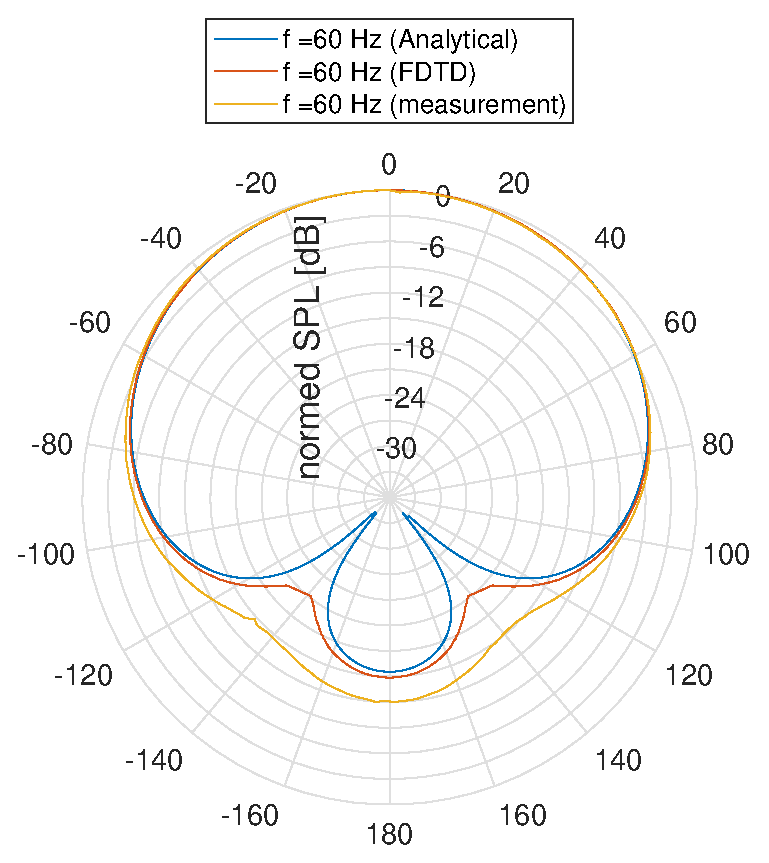
\includegraphics[width=0.85\textwidth]{60_hz_polar_result.eps}
	\caption{Directional characteristics, \SI{60}{\hertz}}
		\label{fig:60_hz_polar_result}
\end{figure}
For a frequency of \SI{100}{\hertz}, results are shown in \autoref{fig:100_hz_polar_result}. Just like at \SI{60}{\hertz}, the augmented analytical model leads to a similar graph to the unaugmented analytical model, while being slightly more optimistic. The graph corresponding to the \gls{fdtd}-based estimate shows slightly less pressure reduction compared to the analytical model everywhere, except arount \SI{\pm 135}{degree}, where it shows significantly less pressure reduction. The measured graph starts deviating from the predicted characteristic closer to \SI{0}{\degree} then it did at \SI{60}{\hertz}. There is less pressure reduction than predicted by all of the models up to angles of approx. \SI{\pm 155}{\degree}. The calculated estimates all show hypercardiod characteristics. Towards the back direction (\SI{180}{\degree}) they predict a lobe, where the estimates range from approx. \SI{14.5}{\decibel} (\gls{fdtd}) to approx. \SI{15.5}{\decibel} attenuation. The measurement result is actually better then this with an attenuation of approx. \SI{17.5}{\decibel} at \SI{180}{\degree}. The shape of the measured graph indicated more of a non-hypercardiod but cardiod characteristic, meaning there is no back lobe. However, there is some asymmetry in the graph with the maximum attenuation of \SI{18}{\decibel} actually reached around \SI{-155}{\degree}.\\
It is hard to declare a winner for \SI{100}{\hertz}, because all estimation approaches actually show a significantly different shape compared to the measurement results. However, when considering the integral over the absolute deviation, the \gls{fdtd}-based approach leads to a smaller error compared to both analytically based approaches. 
\begin{figure}[H]
	\centering
	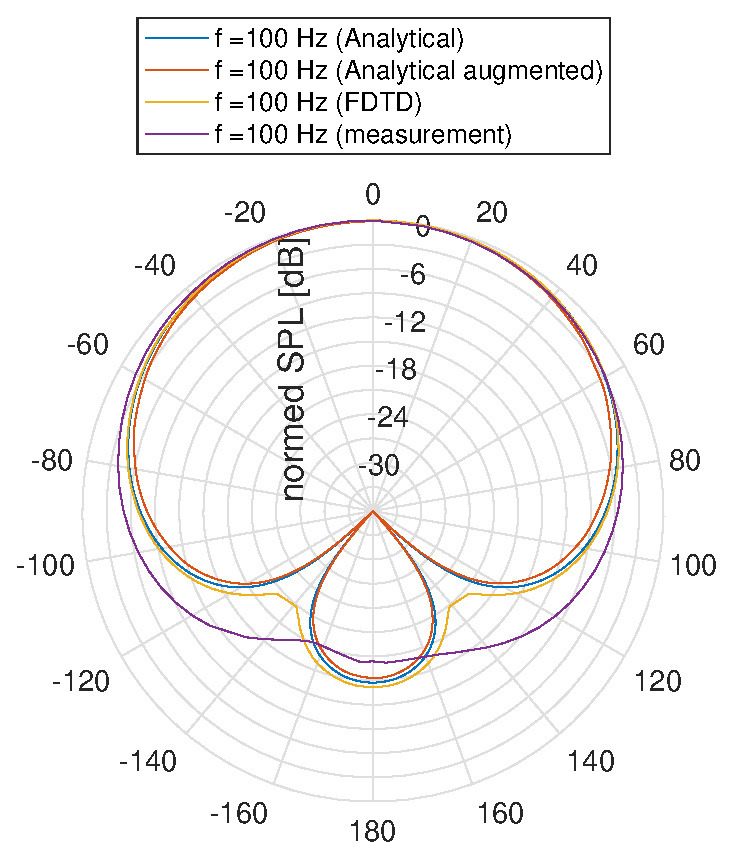
\includegraphics[width=0.85\textwidth]{100_hz_polar_result.eps}
	\caption{Directional characteristics, \SI{100}{\hertz}}
		\label{fig:100_hz_polar_result}
\end{figure}
For a frequency of \SI{150}{\hertz}, results are shown in \autoref{fig:150_hz_polar_result}.
All three calculated estimation approaches behave very similarly to what has been described for the frequencies of \SI{60}{\hertz} and \SI{100}{\hertz}. Opposed to that, the measured characteristics change they shape significantly compared to \SI{100}{\hertz}. The graph is now clearly supercardiod and matches the estimates qualitatively but not quantitatively.
Close to \SI{0}{\degree}, the measured graph matches the unaugmented analytical model and the \gls{fdtd}-based approach well. The pressure drop then is smaller then predicted for bigger angles up to approx. \SI{\pm 150}{\degree}. There are two distinct spikes in the curve, one at approx. \SI{-145}{\degree} that corresponds to an attenuation bigger than \SI{30}{\decibel} and the other one at approx. \SI{150}{\degree} with less attenuation. The back lobe is narrower than predicted. The attenuation at \SI{180}{\degree} is approx. \SI{14}{\decibel}, which matches the value predicted by the unaugmented analytical model almost exactly.\\
At \SI{150}{\hertz} the unaugmented analytical model appears to deliver the closest resembly of the measured graph, because unlike the \gls{fdtd}-based approach it correctly predicts spikes in the attenuation graph. The spikes in the measured graph appear closer to \SI{180}{\degree} than predicted and their magnitude differs from the prediction.
\begin{figure}[H]
	\centering
	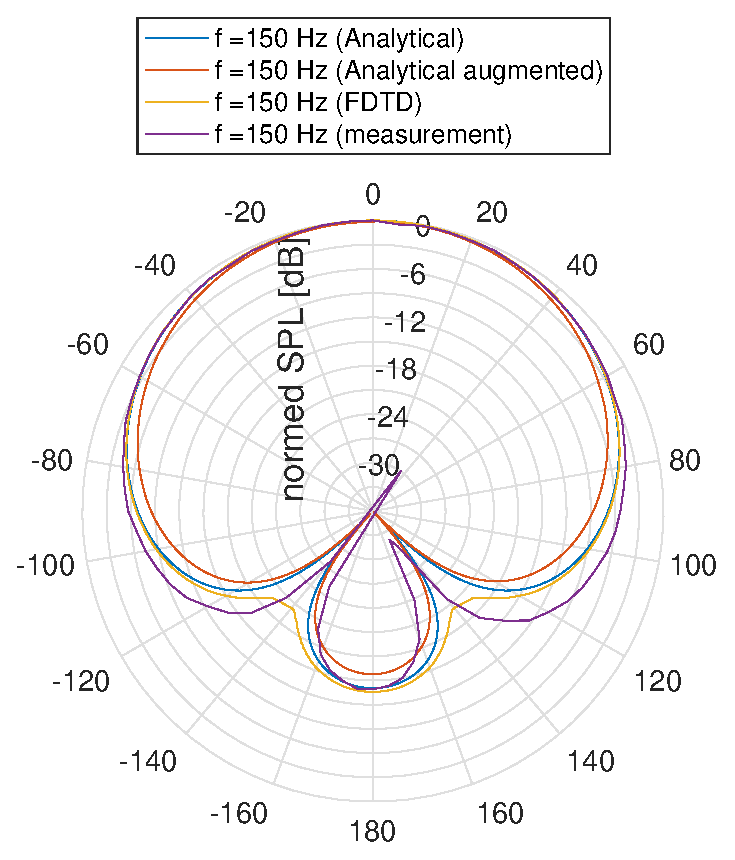
\includegraphics[width=0.85\textwidth]{150_hz_polar_result.eps}
	\caption{Directional characteristics, \SI{150}{\hertz}}
		\label{fig:150_hz_polar_result}
\end{figure}
For a frequency of \SI{200}{\hertz}, results are shown in \autoref{fig:200_hz_polar_result}. Again the calculated predictions show a similar behaviour to what has been described above. It should be noticed, that the augmented analytical model tends to have increasingly ``optimistic'' results compared to the unaugmented model towards higher frequencies, because it takes into account that the loudspeakers in the array have a tendency to behave not perfectly omnidirectional at higher frequencies. This however is not confirmed by the measured graph. It again shows a supercardiod characteristic and matches the predictions well near \SI{0}{\degree} but shows less attenuation towards angles that are further away from the main axis. Similar to \autoref{fig:150_hz_polar_result} at \SI{200}{\hertz} the spikes in the measured graph around approx. \SI{\pm 140}{\degree} are asymmetrical, with the one at approx. \SI{-140}{\degree} peaking at a larger attenuation then the one at approx. \SI{140}{\degree}. The shape of the graph is also asymmetric in the aspect that back lobe is wider towards the positive angles and the smallest attenuation of the back lobe is not at \SI{180}{\degree}, but at \SI{175}{\degree}.
 \begin{figure}[H]
	\centering
	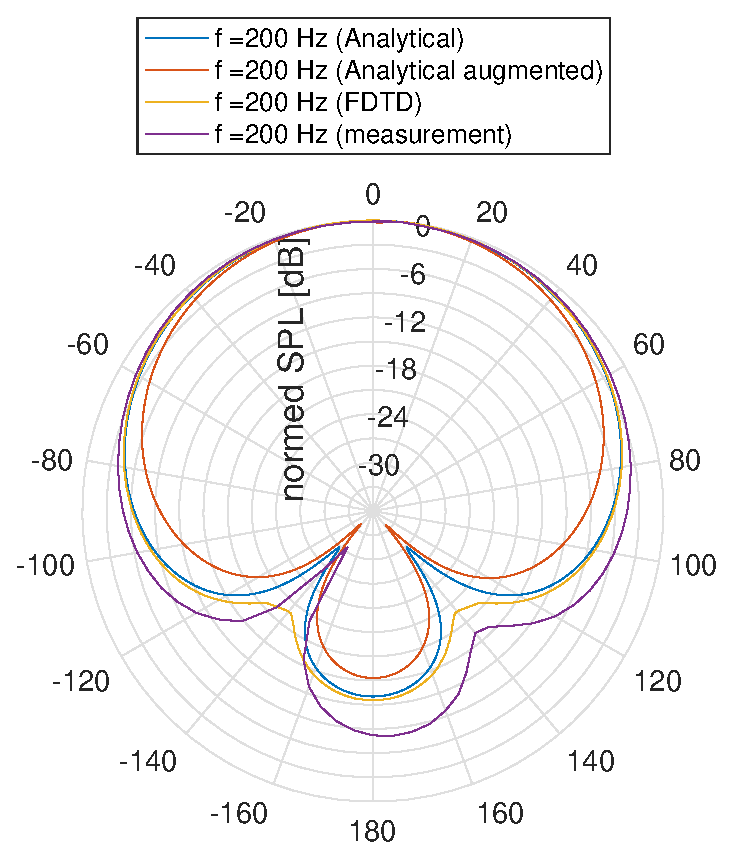
\includegraphics[width=0.85\textwidth]{200_hz_polar_result.eps}
	\caption{Directional characteristics, \SI{200}{\hertz}}
		\label{fig:200_hz_polar_result}
\end{figure}
For a frequency of \SI{250}{\hertz}, results are shown in \autoref{fig:250_hz_polar_result}.

 \begin{figure}[H]
	\centering
	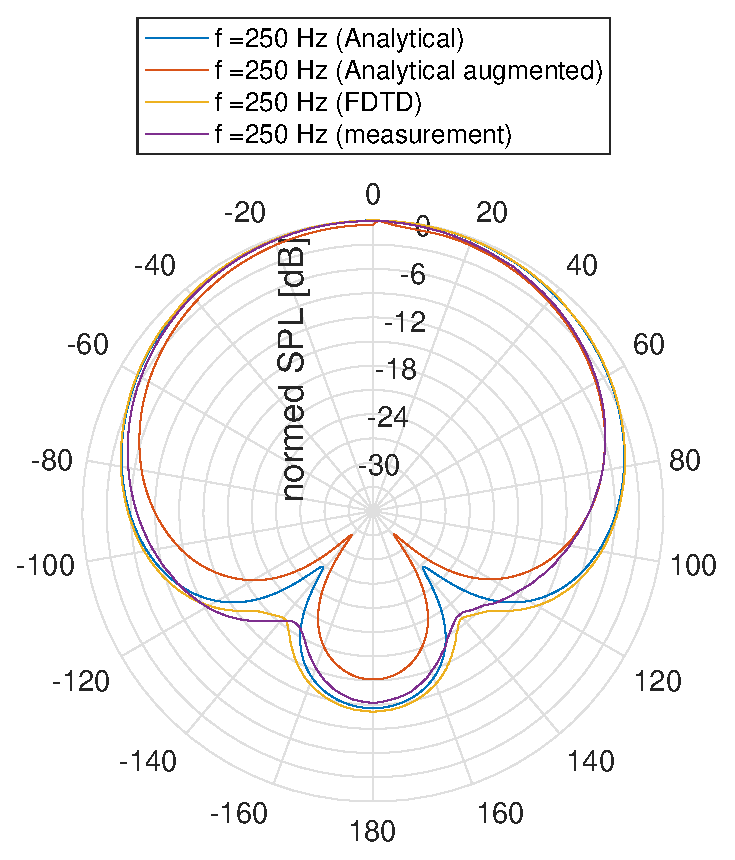
\includegraphics[width=0.85\textwidth]{250_hz_polar_result.eps}
	\caption{Directional characteristics, \SI{250}{\hertz}}
		\label{fig:250_hz_polar_result}
\end{figure}
For a frequency of \SI{300}{\hertz}, results are shown in \autoref{fig:300_hz_polar_result}.
 \begin{figure}[H]
	\centering
	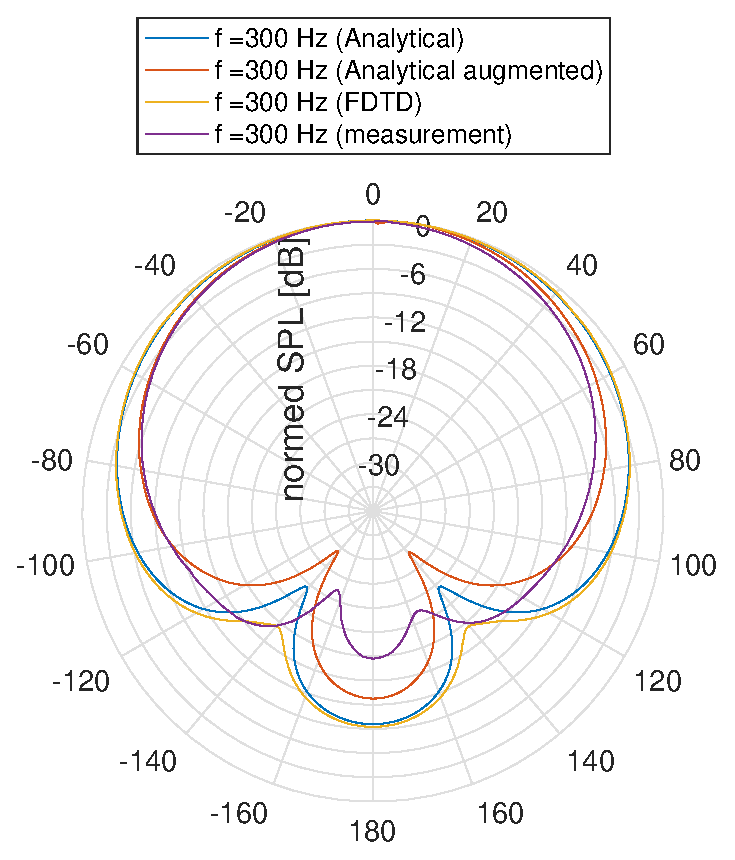
\includegraphics[width=0.85\textwidth]{300_hz_polar_result.eps}
	\caption{Directional characteristics, \SI{300}{\hertz}}
		\label{fig:300_hz_polar_result}
\end{figure}


\section{Conclusion on the Comparison}




